\part{ТФКП}

\section{Криволинейные интегралы от комплекснозначных функций \tpst{"---}{---} определения и свойства}

\begin{definition}
	$ \curvedir \Gamma([a, b]) \sub \R^2, \qquad u, v \in \Cont \Gamma, \qquad u : \Gamma \to \R, \quad v : \Gamma \to \R $ \\
	$ f(x, y) = u(x, y) + iv(x, y) \quad \in \Cont \Gamma $
	$$ \cint[x]{\curvedir \Gamma}{f(x, y)} \define \cint[x]{\curvedir \Gamma}{u(x, y)} + i \cint[x]{\curvedir \Gamma}{v(x, y)} $$
	$$ \cint[y]{\curvedir[0] \Gamma}{f(x, y)} \define \cint[y]{\curvedir[0] \Gamma}{u(x, y)} + i \cint[y]{\curvedir[0] \Gamma}{v(x, y)} $$
\end{definition}

\begin{props}
	\item $ \cint[x]{\curvedir \Gamma}{f + g} = \cint[x]{\curvedir \Gamma}f + \cint[x]{\curvedir \Gamma}g, \qquad \dots \di y $
	\item $ c \in \Co $
	$$ \cint[x]{\curvedir \Gamma}{cf} = c \cint[x]{\curvedir \Gamma}f, \qquad \dots \di y $$
	\item $ \cint[x]{\curvedir[0] \Gamma}f = - \cint[x]{\curvedir \Gamma}f, \qquad \dots \di y $
	\item $ \mathtt T = \seqz[m]{t_\nu}\nu, \quad a = t_0 < \dots < t_m = b, \qquad \mathtt P = \seq[m]{\tau_\nu}\nu, \quad \tau_\nu \in [t_{\nu - 1}, t_\nu] $
	$$ \Gamma(t) =
	\begin{bmatrix}
		x(t) \\
		y(t)
	\end{bmatrix}, \qquad x(t_\nu) \fed x_\nu, \quad y(t_\nu) \fed y_\nu, \qquad M(\tau_\nu) =
	\begin{bmatrix}
		x(\tau_\nu) \\
		y(\tau_\nu)
	\end{bmatrix} $$
	$$ \mathtt S_x(f, \mathtt T, \mathtt P) \define \sum_{\nu = 1}^m f \big( M(\tau_\nu) \big) (x_\nu - x_{\nu - 1}) $$
	$$ \mathtt S_y(f, \mathtt T, \mathtt P) \define \sum_{\nu = 1}^m f \big( M(\tau_\nu) \big) (y_\nu - y_{\nu - 1}) $$
	$$ \forall \eps > 0 \quad \exists \delta > 0 : \quad \forall \mathtt P \quad t_\nu - t_{\nu - 1} < \delta, \quad \nu = 1, \dots, m \quad \implies \bigg| \cint[x]{\curvedir\Gamma}f - \mathtt S_x \bigg| < \eps, \quad \bigg| \cint[y]{\curvedir\Gamma}f - \mathtt S_y \bigg| < \eps $$
	То есть, последовательность сумм Римана сходится к интегралу.
\end{props}

\begin{eproof}
	\item Очевидно.
	\item $ c = a + bi, \qquad f = u + iv $
	$$ cf = au - bv + i(av + bu) $$
	\begin{multline*}
		\cint[x]{\curvedir \Gamma}{cf} = \cint[x]{\curvedir \Gamma}{(au - bv)} + i \cint[x]{\curvedir \Gamma}{(av + bu)} = a \cint[x]{\curvedir \Gamma}u - b \cint[x]{\curvedir \Gamma}v + i \bigg( a \cint[x]{\curvedir \Gamma}v + b \cint[x]{\curvedir \Gamma}u \bigg) = \\
		= a \bigg( \sint[x]u + i \sint[x]v \bigg) + b \bigg( - \sint[x]v + i \sint[x]u \bigg) = a \sint[x]f + bi \sint f = c \sint f
	\end{multline*}
	\item Очевидно.
	\item Следует из аналогичной теоремы для вещественных криволинейных интегралов второго рода.
\end{eproof}

\section{Криволинейные интегралы от комплекснозначных функций и криволинейные интегралы первого рода}

\begin{definition}[криволинейный интеграл второго рода]
	$$ \cint[z]{\curvedir\Gamma}{f(z)} \define \cint[x]{\curvedir\Gamma}{f(z)} + i \cint[y]{\curvedir\Gamma}{f(z)} $$
\end{definition}

\begin{props}
	\item $ \cint[z]{\curvedir\Gamma}{(f + g)} = \cint[z]{\curvedir\Gamma}f + \cint[z]{\curvedir\Gamma}g $

	\item $ \cint[z]{\curvedir\Gamma}{cf} = c \cint[z]{\curvedir\Gamma}f $

	\item $ \cint[z]{\curvedir[0]\Gamma}f = - \int\limits_{\curvedir \Gamma} f \di z $

	\item $ \curvedir\Gamma : z(t), \quad t \in [a, b], \qquad f : \curvedir\Gamma \to \Co, \qquad \mathtt T = \seqz[m]{t_\nu}\nu, \qquad \mathtt P = \seq[m]{\tau_\nu}\nu $
	$$ z_\nu \define z(t_\nu) = x(t_\nu) + iy(t_\nu), \qquad x_\nu \define x(t_\nu), \quad y_\nu \define y(t_\nu), \qquad \hat z_\nu \define z(\tau_\nu) $$
	$$ \mathtt S(f, \mathtt T, \mathtt P) \define \sum_{\nu = 1}^m f(\hat z_\nu) (z_\nu - z_{\nu - 1}) $$
	$ f \in \Cont \Gamma $

	Тогда
	$$ \forall \eps > 0 \quad \exists \delta > 0 : \quad \forall \mathtt T : t_\nu - t_{\nu - 1} < \delta, \quad \nu = 1, \dots, m \quad \forall \mathtt P \quad \bigg| \cint[z]{\curvedir\Gamma}f - \mathtt S(f, \mathtt T, \mathtt P) \bigg| < \eps $$

	\item\label{it:curve_it:5} $ \curvedir\Gamma : [a, b] \to \Co, \qquad z(a) = A, \quad z(b) = B, \qquad c \in \Co $
	$$ \cint[z]{\curvedir\Gamma}c = c(B - A) $$

	\item\label{it:curve_int:6} $ \curvedir \Gamma \sub \Co, \qquad f \in \Cont \Gamma, \qquad c \in \curvedir \Gamma, \qquad \curvedir \Gamma = \curvedir \Gamma_1 \cup \curvedir \Gamma_2, \qquad \curvedir\Gamma_1 \cap \curvedir\Gamma_2 = \set c $
		$$ \cint[z]{\curvedir \Gamma}{f(z)} = \cint[z]{\curvedir\Gamma_1}{f(z)} + \cint[z]{\curvedir\Gamma_2}{f(z)} $$

	\item\label{it:curve_int:7} $ \curvedir\Gamma \sub \Co, \qquad f : \Gamma \to \Co, \qquad f \in \Cont \Gamma, \qquad \Gamma \leftrightarrow \Gamma^* $
	$$ \bigg| \cint[z]{\curvedir\Gamma}{f(z)} \bigg| \le \cint{\Gamma^*}{|f^*(M)|} $$
	В дальнейшем мы будем такой интеграл обозначать $ \acint\Gamma{|f(z)|} $.

	\item\label{it:curve_int:8} $ \curvedir\Gamma \sub \Co, \qquad f \in \Cont \Gamma, \qquad \theta \in (0, 2\pi) $
		$$ \curvedir\Gamma_\theta \define e^{i\theta}\curvedir\Gamma $$
		То есть,
		$$ \curvedir\Gamma_\theta = \set{z \in \Co \mid z = e^{i\theta}\zeta, \quad \zeta \in \Gamma} $$
		$$ f_\theta(z) \define f \big( e^{-i\theta}z), \quad z \in \Gamma_\theta $$
		$$ \implies \cint[\zeta]{\curvedir\Gamma}{f(\zeta)} = e^{-i\theta} \cint[z]{\curvedir\Gamma_\theta}{f_\theta(z)} $$
\end{props}

\begin{eproof}
	\item Очевидно.

	\item $ c = a + bi $
	$$ \cint[z]{\curvedir\Gamma}{cf} \bydef \cint[x]{\curvedir\Gamma}{cf} + i \cint[y]{\curvedir\Gamma}{cf} = c \cint[x]{\curvedir\Gamma}f + ic \cint[y]{\curvedir\Gamma}f = c \bigg( \cint[x]{\curvedir\Gamma}f + i \cint[y]{\curvedir\Gamma}f \bigg) \bydef c \cint[z]{\curvedir\Gamma}f $$

	\item $ \cint[z]{\curvedir[0]\Gamma}f = \cint[x]{\curvedir[0]\Gamma}f + i \cint[y]{\curvedir[0]\Gamma}f = -\int\limits_{\curvedir \Gamma} f \di x - \ii \int\limits_{\curvedir \Gamma} f \di y = -\int\limits_{\curvedir \Gamma} f \di z $

	\item $ \mathtt S(f, \mathtt T, \mathtt P) = \mathtt S_x(f, \mathtt T, \mathtt P) + i \mathtt S_y(f, \mathtt T, \mathtt P) $ \\
	Воспользуемся аналогичным свойством для $ \mathtt S_x, \mathtt S_y $. Пусть
	$$ \bigg| \sint[y]f - \mathtt S_x \bigg| < \frac\eps2, \qquad \bigg| \sint[y]f - \mathtt S_y \bigg| < \frac\eps2 $$
	$$ \bigg| \sint[z]f - \mathtt S \bigg| = \bigg| (\dots x) + i(\dots y) \bigg| \le |\dots x| + |\dots y| < \frac\eps2 + \frac\eps2 = \eps $$

	\item Применим св-во 4. Рассмотрим любые $ \mathtt T, \mathtt P $. \\
	Рассмотрим интегральную сумму
	$$ \mathtt S(c, \mathtt T, \mathtt P) \bydef \sum_{\nu = 1}^m c(z_\nu - z_{\nu - 1}) = c \sum (z_\nu - z_{\nu - 1}) = c(B - A) $$

	\item Докажем для случая, когда $ \Gamma $ "--- гладкая кривая.
	$$ \curvedir\Gamma([a, b]) : [a, b] \to \Co \quad \iff \curvedir\Gamma^*([a, b]) $$
	$$ t \in [a, b], \qquad \Gamma^* : M(t), \qquad M(t) =
	\begin{bmatrix}
		x(t) \\
		y(t)
	\end{bmatrix} $$
	$$ z(t) = x(t) + iy(t) $$
	\begin{multline*}
		\cint[z]{\curvedir \Gamma}{f(z)} = \cint[x]{\curvedir\Gamma^*}{f \big( M(t) \big)} + i \cint[y]{\curvedir\Gamma^*}{f \big( M(t) \big)} = \dint[t]ab{ f^* \big( M(t) \big)x'(t)} + i \dint[t]ab{f^* \big( M(t) \big) y'(t)} = \\
		= \dint[t]ab{ f^* \big( M(t) \big) \big( x'(t) + iy'(t) \big)} = \dint[t]ab{f \big( z(t) \big) \big( x'(t) + iy'(t) \big)} = \\
		= \dint[t]a{t_0}{ f \big( z(t) \big) \big( x'(t) + iy'(t) \big)} + \dint[t]{t_0}b{ f \big( z(t) \big) \big( x'(t) + iy'(t) \big)}
	\end{multline*}
	Прочитывая эти равенства теперь в обратном порядке, получаем, что это равно
	$$ \cint[z]{\curvedir\Gamma_1}{f(z)} + \cint[z]{\curvedir\Gamma_2}{f(z)} $$
	Случай для кусочно-гладких кривых доказывается аналогично.

	\item $ \curvedir\Gamma ([a, b]) \to \Co, \qquad \mathtt T = \seqz[n]{t_j}j, \qquad \mathtt P = \seq[n]{\tau_j}, \qquad z_j = z(t_j), \qquad z_j' = z(\tau_j) $
		$$ \mathtt S (f, \mathtt T, \mathtt P) \bydef \sum_{j = 1}^n f(z_j')(z_j - z_{j - 1}) $$
		$$ |\mathtt S| \le \sum_{j = 1}^n |f(z_j') |z_j - z_{j - 1}| $$
		Перейдём к плоскости $ \R^2 $:
		$$ z(t) = x(t) + iy(t), \qquad M_j =
		\begin{bmatrix}
			x(t_j) \\
			y(t_j)
		\end{bmatrix}, \qquad x_j(t) = x(t_j), \quad y_j = y(t_j) $$
		$$ M_j' =
		\begin{bmatrix}
			x(\tau_j) \\
			y(\tau_j)
		\end{bmatrix}, \qquad x_j' = x(\tau_j), \quad y_j' = y(\tau_j) $$
		$$ \norm{\dist(M_j, M_{j - 1})} = |z_j - z_{j - 1}| $$
		\begin{multline*}
			\| \dist(M_{j - 1} ~ M_{j}) \| \le l \Gamma^*(M_{j - 1}, M_j) \quad \implies \quad \sum_{j = 1}^n |f(z_j')| \cdot |z - z_{j - 1}| \le \\
			\le \sum_{j = 1}^n |f^*(M_j')| \cdot l \Gamma(M_{j - 1}, M_j) \fed \mathtt S^*(|f|, \mathtt T, \mathtt P)
		\end{multline*}
		$$ |\mathtt S| \le \mathtt S^* $$
		Перейдём к пределу:
		$$ \bigg| \cint[z]{\curvedir\Gamma}{f(z)} \bigg| \le \acint\Gamma{|f(z)|} $$

	\item $ \curvedir\Gamma ([a, b]) : [a, b] \to \Co, \qquad \mathtt T = \seqz[n]{t_j}, \quad \mathtt P = \seq[n]{\tau_j}j, \qquad z_j = z(t_j), \quad z_j' = z(\tau_j) $
		\begin{multline*}
			\mathtt S_\Gamma(f, \mathtt T, \mathtt P) \bydef \sum_{j = 1}^n f(z_j')(z_j - z_{j - 1}) = e^{-i\theta} \sum_{j = 1}^n f \bigg( e^{-i\theta}(e^{i\theta}) \bigg) (e^{i\theta}z_j - e^{i\theta}z_{j - 1}) = \\
			= e^{-i\theta} \sum_{j = 1}^n f_\theta(e^{i\theta}z_j')(e^{i\theta}z_j - e^{i\theta}z_{j - 1}) = e^{-i\theta} \mathtt S_{\Gamma_\theta}(f_\theta, \mathtt T, \mathtt P)
		\end{multline*}
\end{eproof}

По индукции из свойства \ref{it:curve_int:6} получаем следующее утверждение:

\begin{property}
	$ c_1, \dots, c_n \in \curvedir\Gamma $
	$$ \cint[z]{\curvedir\Gamma}{f(z)} = \sum_{j = 1}^{n + 1} \int\limits_{\curvedir{\Gamma_j}} f(z) \di z $$
\end{property}

\section{Теорема Коши для прямоугольника}

\begin{theorem}
	$ G \sub \Co, \qquad f \in A(G), \qquad Q = \set{z = x + iy \mid a \le x \le b, \quad p \le y \le q} \sub G $
	$$ \implies \cint[z]{\curvedir{\partial Q}}{f(z)} = 0 $$
\end{theorem}

\begin{note}
	Здесь ориентация роли не играет.
\end{note}

\begin{proof}
	Обозначим
	$$ A = a + pi, \qquad B = b + pi, \qquad C = b + qi, \qquad D = a + qi $$
	$$ \int\limits_{\curvedir{\partial Q}}\dots = \int\limits_{\overrightarrow{AB}} + \int\limits_{\overrightarrow{BC}} + \int\limits_{\overrightarrow{CD}} + \int\limits_{\overrightarrow{DA}} = \bigg( \int\limits_{\overrightarrow{AB}} - \int\limits_{\overrightarrow{DC}} \bigg) + \bigg( \int\limits_{\overrightarrow{BC}} - \int\limits_{\overrightarrow{AD}} \bigg) $$
	Рассмотрим параметризацию $ AB $:
	$$ \overrightarrow{AB} = \set{t + pi \mid t \in [a, b]} $$
	$$ \cint[z]{\overrightarrow{AB}}{f(z)} = \dint[t]ab{f(t + pi)} $$
	Аналогично,
	$$ \overrightarrow{DC} = \set{t + qi}, \qquad \overrightarrow{BC} = \set{b + it}, \qquad \overrightarrow{AD} = {a + ti} $$
	$$ \cint[z]{\overrightarrow{DC}}{f(z)} = \dint[t]ab{f(t + qi)}, \qquad \cint[z]{\overrightarrow{BC}}{f(z)} = i\dint[t]pq{f(b + ti)}, \qquad \cint[z]{\overrightarrow{AD}}{f(z)} = i\dint[t]pq{f(a + ti)} $$
	Всё это означает, что
	\begin{equ}{cauchy_rect:7}
		\cint[z]{\curvedir{\partial Q}}{f(z)} = \bigg( \dint[t]ab{f(t + pi)} - \dint[t]ab{f(t + qi)} \bigg) + \bigg( i \dint[t]pq{f(b + ti)} - i\dint[t]pq{f(a + ti)} \bigg)
	\end{equ}
	Перейдём к плоскости $ \R^2 $:
	$$ \dint[t]ab{f^*(t, q)} - \dint[t]ab{f^*(t, p)} = \dint[x]ab{ \bigg( f^*(x, q) - f^*(x, p) \bigg) } $$
	$ f^* \in \Cont[1]{G^*} $, значит, можно применить формулу Ньютона"--~Лейбница:
	$$ = \dint ab{ \bigg( \dint[y]pq{f_y^*{}'(x, y)} \bigg)} $$
	Аналогично,
	$$ \dint[y]pq{f^*(b, y) - f^*(a, y)} = \dint[y]pq{ \bigg( \dint ab{f_x^*{}'(x, y)} \bigg) } $$
	Подставляя последние две выкладки в \eref{cauchy_rect:7}, получаем
	\begin{multline*}
		\cint[z]{\curvedir{\partial Q}}{f(z)} = -\dint ab{ \dint[y]pq{ f_y^*{}'(x, y)}} + i \dint[y]pq{ \dint ab{f_x^*{}'(x, y)}} = \\
		= \dint ab{ \dint[y]pq{ -f_y^*{}' + if_x^*{}'}} = 2i \dint ab{ \dint[y]pq {\frac12 \bigg( f_x^*{}' + if_x^*{}' \bigg)}} \bydef 2i \dint ab { \dint[y]pq{ \underbrace{f_{\ol z}'}_0}} = 0
	\end{multline*}
\end{proof}

\section{Теорема Коши для прямоугольного треугольника}

\begin{figure}[!h]
	\centering
	\begin{subfigure}{0.4\textwidth}
		\centering
		\begin{tikzpicture}[>=Stealth]
			\draw (1, 1) -- (3, 3) node[right] {$ C $};
			\draw (1, 1) -- (3, 1) node[right] {$ B $};
			\draw (3, 1) -- (3, 3);
			\draw (1, 1) node[below] {$ A $};

			\draw (2, 1) node[below] {$ K $};
			\draw (3, 2) node[right] {$ E $};
			\draw (2, 2) node[left] {$ D $};
			\draw (2, 1) -- (2, 2) -- (3, 2);

			\draw (1.75, 1.25) node {$ \vartriangle_2 $};
			\draw (2.75, 2.25) node {$ \vartriangle_1 $};
		\end{tikzpicture}
		\caption{Прямоугольный треугольник}
		\label{pic:1a}
	\end{subfigure}
	\begin{subfigure}{0.4\textwidth}
		\centering
		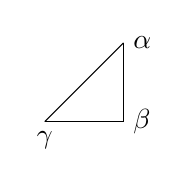
\begin{tikzpicture}
			\draw (0, 0) -- (1, 1) node[right] {$ \alpha $};
			\draw (0, 0) -- (1, 0) node[right] {$ \beta $};
			\draw (1, 0) -- (1, 1);
			\draw (0, 0) node[below] {$ \gamma $};
		\end{tikzpicture}
		\caption{Прямоугольный треугольничек}
		\label{pic:1b}
	\end{subfigure}
\end{figure}

\begin{theorem}
	Рассматриваем треугольник $ ABC $ (\autoref{pic:1a}).
	$$ f \in \mathcal A(G), \qquad A = a + pi, \quad B = b + pi, \quad c = b + qi, \qquad a < b, \quad p < q, \qquad \vartriangle ABC \sub G $$
	$$ I \define \cint[z]{\curvedir{\partial \vartriangle} ABC}{f(z)} = 0 $$
\end{theorem}

\begin{proof}
	Рассмотрим точки:
	$$ D = \frac{a + b}2 + i \frac{p + q}2, \qquad K = \frac{a + b}2 + pi, \qquad E = b + i \frac{p + q}2 $$
	$$ \cint[z]{\curvedir{\partial \vartriangle} ABC}{f(z)} = \int\limits_{\curvedir{\partial \Box}} + \int\limits_{\curvedir{\partial \vartriangle_1}} + \int\limits_{\curvedir{\partial \vartriangle_2}} $$
	При этом,
	$$ \int\limits_{\overrightarrow{ED}} + \int\limits_{\overrightarrow{DE}} = 0, \qquad \int\limits_{\overrightarrow{DK}} + \int\limits_{\overrightarrow{KD}} = 0 $$
	К каждому из треугольников можно применить такое же рассуждение, а к прямоугольникам "--- теорему Коши для прямоугольника. Получаем
	\begin{equ}{cauchy_rect_trian:1}
		I = \sum_{k = 1}^{2^n} I_{n_k}
	\end{equ}
	$$ I_{n_k} = \cint[z]{\curvedir{\partial \vartriangle_{n_k}}}{f(z)} $$
	Рассмотрим какой-то из шагов (треугольник обозначим $ \alpha\beta\gamma $, \autoref{pic:1b}):
	$$ \cint[z]{\curvedir{\partial \vartriangle}\alpha\beta\gamma}{f(z)} = \cint[z]{\curvedir{\partial\vartriangle}\alpha\beta\gamma}{f(z) - f(\alpha)} + f(\alpha) \cint[z]{\curvedir{\partial\vartriangle}\alpha\beta\gamma}1 $$
	Второй интеграл равен 0 (по св-ву \ref{it:curve_it:5} криволинейных интегралов). Значит, это равно
	$$ \cint[z]{\curvedir{\partial\vartriangle}\alpha\beta\gamma}{f(z) - f(\alpha)} $$
	По св-ву \ref{it:curve_int:7} криволинейных интегралов, это означает, что
	\begin{equ}{cauchy_rect_trian:4}
		\bigg| \cint[z]{\curvedir{\partial\vartriangle}\alpha\beta\gamma}{f(z)} \bigg| \le \acint{\partial\vartriangle\alpha\beta\gamma}{|f(z) - f(\alpha)|}
	\end{equ}
	Применим теорему Кантора:
	$$ \forall \eps > 0 \quad \exists \delta > 0 : \quad \forall \alpha \in [A, C], \quad z \in \partial \vartriangle \alpha\beta\gamma \quad |f(z) - f(\alpha)| < \eps $$
	Выберем $ n $ так, что
	$$ z^{-n} \cdot |C - A| < \delta $$
	Тогда
	$$ \acint{\partial \vartriangle\alpha\beta\gamma}{|f(z) - f(\alpha)|} < \eps \acint{\partial\vartriangle\alpha\beta\gamma}{} \underset{\text{из геом. сообр.}}< 3\eps |\gamma - \alpha| = 3\eps \cdot |C - A| \cdot 2^{-n} $$
	$$ \underimp{\eref{cauchy_rect_trian:4}} \forall k \quad |I_{n_k}| < 3 \eps |C - A| \cdot 2^{-n} $$
	$$ \underimp{\eref{cauchy_rect_trian:1}} |I| \le \sum_{k = 1}^{2^n}|I_{n_k} < 3\eps |C - A| \cdot 2^{-n} \cdot 2^n = 3 \eps |C - A| $$
	$$ \implies |I| = 0 $$
\end{proof}

Если треугольник перевернуть относительно оси ординат, результат не изменится.

\begin{remark}
	Аналитичность $ f $ использовалась для прямоугольника.
\end{remark}

\section{Теорема Коши для произвольного треугольника}

\begin{figure}[!ht]
	\centering
	\begin{subfigure}{0.4\textwidth}
		\centering
		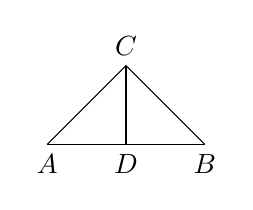
\begin{tikzpicture}
			\draw (0, 0) -- (2, 0) node[below] {$ B $};
			\draw (0, 0) -- (1, 1) node[above] {$ C $};
			\draw (1, 1) -- (1, 0) node[below] {$ D $};
			\draw (0, 0) node[below] {$ A $};
			\draw (2, 0) -- (1, 1);
		\end{tikzpicture}
		\caption{}
		\label{pic:2}
	\end{subfigure}
	\begin{subfigure}{0.4\textwidth}
		\centering
		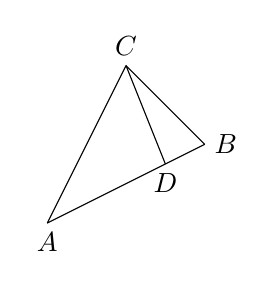
\begin{tikzpicture}
			\draw (0, 0) node[below] {$ A $};
			\draw (0, 0) -- (2, 1) node[right] {$ B $};
			\draw (0, 0) -- (1, 2) node[above] {$ C $};
			\draw (1, 2) -- (1.5, 0.75) node[below] {$ D $};
			\draw (1, 2) -- (2, 1);
		\end{tikzpicture}
		\caption{}
		\label{pic:3}
	\end{subfigure}
\end{figure}

\begin{theorem}
	Рассматриваем треугольник $ ABC $ (\autoref{pic:2})
	$$ A = a + pi, \quad B = b + pi, \quad C = d + qi, \qquad a < d < l, \qquad q > p $$
	$$ \underbrace{\int\limits_{\curvedir{\partial \vartriangle}ADC}}_0 + \underbrace{\int\limits_{\curvedir{\partial\vartriangle}DBC}}_0 = \int\limits_{\curvedir{\partial\vartriangle}ABC} = 0 $$
\end{theorem}

\begin{theorem}
	Рассматриваем треугольник $ ABC $ (\autoref{pic:3}). Считаем, что наибольшая сторона "--- это $ AB $.

	Возьмём $ \theta $ так, что $ e^{i\theta} \cdot \vartriangle ABC $ повёрнут ``правильно''.
	$$ f_\theta(z) \define f(e^{-i\theta}z), \qquad f_\theta \in A(G_\theta) $$
	Получаем треугольник $ A_1B_1C_1 $ из предыдущей теоремы.

	Дальше пользуемся свойством \ref{it:curve_int:8} криволинейных интегралов.
\end{theorem}

\section{Теорема Коши для многоугольника}

\begin{theorem}
	Имеется некая конечносвязная многоугольная область $ D $, ограниченная многоугольниками $ \Gamma_1, \dots, \Gamma_k $.
	$$ \partial D = \bigcup_{\nu = 1}^k \Gamma_\nu $$
	Пусть есть область $ G $ такая, что $ G \supset \ol D $ и функция $ f \in \mathcal A(G) $. Рассмотрим
	$$ \curvedir \partial D = \bigcup_{\nu = 1}^k \curvedir \Gamma_\nu, $$
	при этом, каждая кривая $ \Gamma_\nu $ положительно ориентированна относительно области $ D $.
	$$ \implies \cint[z]{\curvedir\partial D}{f(z)} = 0 $$
\end{theorem}

\begin{proof}
	Применим теорему о триангуляции конечносвязной многоугольной области:
	$$ \exists \seq[N]{\Delta_k}k, \quad \Delta_k \text{ "--- откр.: } \qquad
	\begin{cases}
		\Delta_k \cap \Delta_l = \O, \quad k \ne l \\
		\ol\Delta_k \cap \ol\Delta_l =
		\begin{cases}
			\O \\
			\text{общая вершина} \\
			\text{общая сторона}
		\end{cases} \\
		\bigcup_{k = 1}^N \ol \Delta_k = \ol D
	\end{cases} $$
	Рассмотрим
	$$ \sum_{k = 1}^N \cint[z]{\curvedir{\partial\Delta}_k}{f(z)} $$
	Каждый из них представим в виде суммы интегралов по трём сторонам. В результате:
	\begin{enumerate}
		\item каждый внутренний отрезок мы пройдём дважды в разных направлениях;
		\item все ``внутренние'' границы (многоугольники) проходятся полностью в отрицательном (относительно внешнего многоугольника) направлении;
		\item остаётся только ``внешняя'' граница.
	\end{enumerate}
	$$ \sum = 0 $$
\end{proof}

\section{Лемма об оценке интеграла}

\begin{figure}[!h]
	\centering
	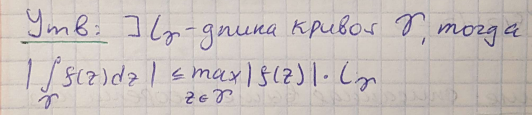
\includegraphics[width=0.75\textwidth]{integral_lemma}
	\caption{Лемма из конспектов прошлых лет.}
	\label{fig:integral_lemma}
\end{figure}

\begin{note}
	Эту лемму я найти не смог, так что исхожу из предположения, что она отдельно не выделялась и спрятана в следующей теореме.
	Также, предполагаю, что на \autoref{fig:integral_lemma} приведена эта лемма\footnote{\href{https://drive.google.com/drive/folders/1yCcFWKQGFlAZvy61gvlXTFQ4SfuWRc6I}{Источник}. Низкий поклон этим людям.}.
	Возможно, лемма об оценке интеграла "--- это вообще другое.
\end{note}

\begin{lemma}
	$$ \Bigl| \int\limits_{\curvedir \Gamma} f(z) \di z \Bigr| \le \max\limits_{z \in \Gamma} |f(z)| \cdot l \Gamma $$
\end{lemma}

\begin{proof}
	По свойству \ref{it:curve_int:7} криволинейных интегралов,
	$$ \Bigl| \int\limits_{\curvedir \Gamma} f(z) \di z \Bigr| \le \int\limits_\Gamma |f(z)|~|\di z| \le \int\limits_\Gamma \max |f(z)|~|\di z| \underset{\text{св-во \ref{it:curve_int:6}}}\le \max |f(z)| \cdot l \Gamma $$
\end{proof}

\section{Теорема Коши для области с кусочно-гладкими границами}

\begin{theorem}
	$ G \sub \Co, \qquad \ol D \sub G, \qquad \partial D = \bigcup_{k = 1}^m \Gamma_k, \qquad \Gamma_k $ кусочно-гладкие, $ \qquad f \in \mathcal A(G) $
	$$ \cint[z]{\curvedir\partial D}{f(z)} = 0 $$
\end{theorem}

\begin{proof}
	Пусть $ \Gamma_k : [a, b] \to \Co $.
	$$ \exists \delta_0 > 0 : \quad \forall \zeta \in \partial D \quad \ol{\mathtt B}(\zeta) = \set{ z \mid |z - \zeta| \le \delta_0} \sub G $$
	$$ T_{\delta_0} \define \bigcup_{\zeta \in \partial D} \ol{\mathtt B_{\delta_0}(\zeta)} $$
	\begin{statement}
		$ T_{\delta_0} $ "--- компакт.
	\end{statement}
	\begin{proof}
		Упражнение.
	\end{proof}
	Значит, по теореме Кантора, \\
	$ f \in \Cont{T_{\delta_0}} \implies f $ равномерно непрерывна на $ T_{\delta_0} $. То есть,
	\begin{equ}{cauchy_domain:1}
		\forall \eps > 0 \quad \exists 0 < \delta_1 \le \delta_0 : \quad \forall z_1, z_2 \in T_{\delta_0} : |z_1 - z_2| < \delta_1 \quad |f(z_1) - f(z_2)| < \eps
	\end{equ}
	Обозначим $ \mathtt P_k = \seqz[N_k]{t_{kj}}j, \quad t_{k0} = a_k, \quad t_{kN_k} = b_k, \quad k = 1, \dots, m $. \\
	Выберем его так, чтобы
	$$ \forall t \in [t_{kj}, t_{k~j + 1}] \quad |\Gamma(t) - \Gamma(t_{kj})| < \delta_1 $$
	Такое разбиение можно выбрать в силу равномерной непрерывности.

	Обозначим многоугольник $ S_k = \seqz[M_k]{\Gamma(t_{kj})}j $.

	Обозначим $ \vawe D $ так, что $ \partial \vawe D = \bigcup_{k = 1}^m S_k $. По определению $ \vawe D \sub G $. Применим к $ \vawe D $ аналогичную теорему для многоугольников:
	\begin{equ}{cauchy_domain:5}
		\cint[z]{\curvedir\partial\vawe D}{f(z)} = 0 \quad
		\implies \quad \cint[z]{\curvedir[0]\partial\vawe D}{f(z)} = 0 \quad
		\implies \quad \cint[z]{\curvedir\partial D}{f(z)} = \cint[z]{\curvedir\partial D}{f(z)} + \cint[z]{\curvedir[0]\partial\vawe D}{f(z)}
	\end{equ}
	Рассмотрим некоторую кривую $ \Gamma_k $ (ориентация согласована с общей ориентацией границы). \\
	Обозначим $ \Gamma(t_{kj}) \fed z_{kj}, \quad 0 \le j \le N_k $.

	Рассмотрим случай, когда $ k = 1 $ (остальные "--- аналогично). Это внешняя кривая. \As кривая замкнутая, $ z_{k0} = z_{kN_k} $.

	Рассмотрим точки $ z_{1j}, z_{1~j + 1}, z_{1~j + 2} $. Они обходятся в положительном направлении. Но, если рассматривать многоугольник $ S_1 $, то на нём эти же точки обходятся в противоположном направлении.

	Обозначим $ \curvedir\gamma_{1j} \define \Gamma([t_{1j}, t_{1~j + 1}]) $. По одному из свойств,
	$$ \cint[z]{\curvedir\Gamma_1}{f(z)} = \sum_{j = 0}^{N_1 - 1} \cint[z]{\curvedir{\gamma_{1j}}}{f(z)} $$
	Обозначим $ \sigma_{1j} $ "--- отрезок с концами $ z_{1j}, z_{1~j + 1} $. Тогда
	$$ \cint[z]{\curvedir[0] {S_1}}{f(z)} = \sum_{j = 0}^{N_1 - 1} \cint[z]{\curvedir[0]{\sigma_{1j}}}{f(z)} $$
	Из последних двух выражений получаем, что
	\begin{equ}{cauchy_domain:7'}
		\cint[z]{\curvedir{\Gamma_1}}{f(z)} + \cint[z]{\curvedir[0]{S_1}}{f(z)} = \sum_{j = 0}^{N_1 - 1} \bigg( \cint[z]{\curvedir{\gamma_{1j}}}{f(z)} + \cint[z]{\curvedir[0]{\sigma_{1j}}}{f(z)} \bigg)
	\end{equ}
	Возьмём $ c \in \Co $.
	$$ \cint[z]{\curvedir{\gamma_{1j}}}c + \cint[z]{\curvedir[0]{\sigma_{1j}}}c = c(z_{1~j + 1} - z_{1j}) + c(z_{1j} - z_{1~j + 1}) = 0 \quad \forall c $$
	Пусть теперь $ c = -f(z_{1j}) $
	\begin{equ}{cauchy_domain:9}
		\eref{cauchy_domain:7'} = \sum_{j = 0}^{N_1 - 1} \bigg( \cint[z]{\curvedir{\gamma_{1j}}}{ \big( f(z) - f(z_{1j}) \big) } + \cint[z]{\curvedir[0]{\sigma_{1j}}}{\big( f(z) - f(z_{1j}) \big) } \bigg)
	\end{equ}
	При $ z \in \gamma_{1j} $ и $ z \in \sigma_{1j} $ можно применить лемму:
	$$ \Bigl| \int\limits_{\curvedir{\gamma_{1j}}} f(z) - f(z_{1j}) \di z \Bigr| \le \eps \cdot l \gamma_{1j}, \quad \Bigl| \int\limits_{\curvedir{\sigma_{1j}}} f(z) - f(z_1) \di z \Bigr| \le \eps \cdot l \sigma_{1j} $$

	$$ \implies \bigg| \cint[z]{\curvedir{\gamma_{1j}}}{f(z)} + \cint[z]{\curvedir[0]{\sigma_{1j}}}{f(z)} \bigg| < 2\eps \cdot l ~ \gamma_{1j} $$
	$$ \underimp{\eref{cauchy_domain:9}} \bigg| \cint[z]{\curvedir{\Gamma_1}}{f(z)} + \cint[z]{\curvedir[0]{S_1}}{f(z)} \bigg| < 2\eps \sum_{j = 0}^{N_1 - 1} l ~ \gamma_{1j} = 2 \eps l \Gamma_1 $$
	При остальных $ k $ "--- аналогично.

	$$ \underimp{\eref{cauchy_domain:5}} \bigg| \cint[z]{\curvedir\partial D}{f(z)} \bigg| < 2\eps \sum l \Gamma_k \quad
	\implies \quad \cint[z]{\curvedir\partial D}{f(z)} = 0 $$
\end{proof}

\section{Формула Коши для функции, аналитической в круге}

\begin{theorem}
	$ G \sub \Co, \qquad D = \mathtt B_r(z_0), \qquad \ol D \sub G, \qquad f \in \mathcal A(G), \qquad z \in D $
	\begin{equ}{cauchy_formula:21}
		f(z) = \frac1{2\pi i} \cint[\zeta]{\curvedir\partial D}{\frac{f(\zeta)}{\zeta - z}}
	\end{equ}
\end{theorem}

\begin{figure}[!h]
	\begin{tikzpicture}
		\draw[dashed] (0, 0) circle[radius=3];
		\fill (0, 0) circle[radius=0.03] node[below] {$ z_0 $};
		\draw (0, 0) -- (-3, 0);
		\node at (-1, 0) [below]{$ r $};
		\node at (3, 0) [left]{$ D $};
		\node at (3, 0) [right]{$ S $};

		\draw[dashed] (1, 1) circle[radius=1];
		\fill (1, 1) circle[radius=0.03] node[below] {$ z $};
		\draw (1, 1) -- (0, 1);
		\node at (0.5, 1) [below]{$ \delta $};
		\node at (2, 1) [right]{$ \sigma_\delta $};

		\fill[even odd rule, pattern=dots, pattern color=black!30!white] (0, 0) circle[radius=3] (1, 1) circle[radius=1];
		\node at (0, -1.5) {$ D_\delta $};
	\end{tikzpicture}
	\caption{Картинка к доказательству}
\end{figure}

\begin{proof}
	Возьмём $ \delta > 0 $ так, чтобы $ \delta < r - |z - z_0| $. \\
	Рассмотрим $ \mathtt B_\delta = \set{\zeta \mid |\zeta - z| < \delta} $. Понятно, что $ \ol{\mathtt B}_\delta \sub D $.

	Рассмотрим
	$$ \vphi(\zeta) = \frac{f(\zeta)}{\zeta - z} $$
	Она аналитична в $ D \setminus \set{z} $.

	Рассмотрим область $ D_\delta = D \setminus \ol{\mathtt B}_\delta $.
	$$ \ol D_\delta \sub G \setminus \set z $$
	По теореме Коши,
	\begin{equ}{cauchy_formula:23}
		\cint[\zeta]{\curvedir\partial D_\delta}{\vphi(\zeta)} = 0
	\end{equ}
	Обозначим $ S = \set{\zeta \mid |\zeta - z_0| = r}, \quad \sigma_\delta = \set{\zeta \mid |\zeta - z| = \delta} $.
	$$ \eref{cauchy_formula:23} \implies \cint[\zeta]{\curvedir S}{\vphi(\zeta)} + \cint[\zeta]{\curvedir[0]{\sigma_\delta}}{\phi(\zeta)} = 0 \quad \iff \quad \cint[\zeta]{\curvedir S}{\vphi(\zeta)} = - \cint[\zeta]{\curvedir[0]{\sigma_\delta}}{\vphi(\zeta)} = \cint[\zeta]{\curvedir{\sigma_\delta}}{\vphi(\zeta)} $$
	\begin{equ}{cauchy_formula:26}
		\cint[\zeta]{\curvedir{\sigma_\delta}}{\frac{f(z)}{\zeta - z}} = f(z) \cint[\zeta]{\curvedir{\sigma_\delta}}{\frac1{\zeta - z}}
	\end{equ}
	$$ \curvedir{\sigma_\delta} = \set{\zeta \mid \zeta = z + \delta e^{i\theta}, \quad \theta \in [0, 2\pi]} $$
	$$ \bigg( \delta e^{i\theta} \bigg)_\theta' = i \delta e^{i\theta} $$
	$$ \cint[\zeta]{\curvedir{\sigma_\delta}}{\frac1{\zeta - z}} = \dint[\theta]0{2\pi}{\frac{\big( \delta e^{i\theta} \big)'}{\delta e^{i\theta}}} = 2\pi i $$
	\begin{equ}{cauchy_formula:29}
		\underimp{\eref{cauchy_formula:26}} \cint[\zeta]{\curvedir{\sigma_\delta}}{\frac{f(z)}{\zeta - z}} = 2\pi i f(z)
	\end{equ}
	В силу непрерывности
	$$ \forall \eps > 0 \quad \exists \delta > 0 : \quad \forall \zeta \in \sigma_\delta \quad |f(\zeta) - f(z)| < \eps $$
	$$ \bigg| \cint[\zeta]{\curvedir{\sigma_\delta}}{\frac{f(\zeta) - f(z)}{\zeta - z}} \bigg| \le \acint[\zeta]{\sigma_\delta}{\frac{|f(\zeta) - f(z)|}{|\zeta - z|}} \le \acint[\zeta]{\sigma_\delta}{\frac\eps\delta} = \frac\eps\delta \cdot 2\pi \delta = 2\pi \eps $$
	$$ \bigg| \cint[\zeta]{\curvedir S}{ \frac{f(\zeta)}{\zeta - z}} - 2 \pi i f(z) \bigg| \undereq{\eref{cauchy_formula:29}} \bigg| \cint[\zeta]{\curvedir{\sigma_\delta}}{\frac{f(\zeta) - f(z)}{\zeta - z}} \bigg| \le 2\pi \eps $$
	$$ \implies \cint[\zeta]{\curvedir S}{\frac{f(\zeta)}{\zeta - z}} - 2\pi i f(z) = 0 $$
\end{proof}

\section{Бесконечная гладкость аналитической функции}

\begin{remark}[о предстоящем рассуждении]
	$$ f_z' = \frac12(f_x' - if_y'), \qquad f_{\ol z}' = \frac12(f_x' + if_y') = 0 $$
	$$ f' = f_z' = f'_z + f_{\ol z}' = f_x', \qquad f' = f_z' = f_z' - f_{\ol z}' = if_y' $$
	$$ f_y' = if' $$
	$$ z^\alpha, \qquad z \in \Co \setminus (-\infty, 0], \qquad \alpha \in \Co $$
	$$ z^\alpha \bydef e^{\alpha \ln z} $$
	$ z^n, \quad n \in \N $ определено при $ z \in \Co $ \\
	$ z^{-n} $ определено при $ z \in \Co \setminus \set 0 $
	$$ (z^n)' = nz^{n - 1} $$
	$$ (z^{-n})' = -nz^{-n - 1} $$
	$$ \bigg( (z - a)^{-n} \bigg)' = -n(z - a)^{-n - 1} $$
	$$ \bigg( (z - a)^{-n} \bigg)_x' = -n(z - a)^{-n - 1}, \qquad \bigg( (z - a)^{-n} \bigg)_y' = -in(z - a)^{-n - 1} $$
	$$ \bigg( \frac1{z - a} \bigg)_x' = - \frac1{(z - a)^2}, \qquad \bigg( \frac1{z - a} \bigg)_y' = -i \frac1{(z - a)^2} $$
	$$ \implies \bigg( \frac1{a - z} \bigg)_x' = \frac1{(a - z)^2}, \qquad \bigg( \frac1{a - z} \bigg)_y' = \frac{i}{(a - z)^2} $$
	$$ \bigg( \frac1{a - z} \bigg)_{xx}'' = \bigg( \frac1{(a - z)^2} \bigg)_x' = \frac2{(a - z)^3}, \qquad \bigg( \frac1{a - z} \bigg)_{xy}'' = i \bigg( \frac1{(a - z)^2} \bigg) = \frac{2i}{(a - z)^3} $$
	$$ \bigg( \frac1{a - z} \bigg)_{yy}'' = i \bigg( \frac1{(a - z)^2} \bigg)_y' = \frac{2i^2}{(a - z)^3} $$
	$$ \widedots[5cm] $$
	\begin{equ}{infinite_smooth:21}
		\bigg( \frac1{a - z} \bigg)_{\underbrace{x \dots x}_m \underbrace{y \dots y}_n} = \frac{(m + n)!i^n}{(a - z)^{m + n + 1}}
	\end{equ}
\end{remark}

\begin{theorem}
	$ D \sub \Co, \qquad f \in \mathcal A (D) \qquad \implies \qquad f \in \Cont[\infty] D $
\end{theorem}

\begin{eproof}
	\item $ D = \set{z \mid |z - a| < R} $

	Выберем $ 0 < \rho < R $ и $ \rho < r < R $. Обозначим $ S = \set{z \mid |z - a| = r} $. Применим формулу Коши:
	$$ f(z) = \frac1{2\pi i} \cint[\zeta]{\curvedir S}{\frac{f(\zeta)}{\zeta - z}} $$
	При этом, $ S = \set{z = a + re^{i\theta}} $. Значит,
	$$ f(z) = \frac1{2\pi i} \dint[\theta]0{2\pi}{\frac{f(a + re^{i\theta})}{{a + re^{i\theta} - z}}ire^{i\theta}} $$
	При этом, $ z = x + iy $.
	\begin{statement}
		Теоремы о непрерывности интегралов от параметра и о производной интеграла от параметра остаются справедливыми, если функции комплекснозначные, а параметров несколько.
	\end{statement}
	Применим их и воспользуемся формулой \eref{infinite_smooth:21}:
	\begin{multline*}
		\bigg( f(z) \bigg)_{\underbrace{x \dots x}_m \underbrace{y \dots y}_n}^{(m + n)} = (m + n)!i^n \cdot \frac1{2\pi i} \dint[\theta]0{2\pi}{\frac{f(a + re^{i\theta})ir}{(a + re^{i\theta} - z)^{m + n + 1}}} = \\
		= (m + n)!i^n \cdot \frac1{2\pi i} \cint[\zeta]{\curvedir S}{\frac{f(\zeta)}{(\zeta - z)^{m + n + 1}}}
	\end{multline*}
	$$ \implies \big( f(z) \big)_{\underbrace{x \dots x}_m \underbrace{y \dots y}_n}^{(m + n)} \in \Cont{ \set{z \mid |z - a| \le \rho }} $$
	В силу произвольности $ \rho $ это означает, что $ f \in \Cont[m + n]{\set{z \mid |z - a| < R}} $. \\
	Значит, $ f \in \Cont[\infty]{|z - a| < R} $.

	\item Произвольная область $ D \sub \Co $

	Возьмём $ a \in D $
	$$ \exists R : \quad \set{z \mid |z - a| < R} \sub D $$
	По только что доказанному $ f \in \Cont[\infty]{\set{ z \mid |z - a| < R}} $.

	Поскольку класс $ \mathcal C^\infty $ определяется локально, теорема доказана.
\end{eproof}

\section{Аналитичность производной аналитичной функции}

\begin{theorem}
	$ D \sub \Co, \qquad f \in \mathcal A(D) \qquad \implies \qquad f' \in A(D) $
\end{theorem}

\begin{proof}
	$ f' = f_x' $

	У $ f $ были все производные, а значит, и у $ f_x' $ есть все производные, то есть $ f' \in \Cont[\infty]D $.

	\begin{enumerate}
		\item Рассмотрим $ D = \set{z \mid |z - a| < R}, \quad 0 < \rho < r < R $.
			$$ f(z) = \frac1{2\pi i} \cint[\zeta]{\curvedir S}{\frac{f(\zeta)}{\zeta - z}} $$
			$$ f'(z) = f_x'(z) = \frac1{2\pi i} \cint[\zeta]{\curvedir S}{\frac{f(\zeta)}{(\zeta - z)^2}} $$
			Применим формулу \eref{infinite_smooth:21}:
			$$ \left.
				\begin{aligned}
					\big( f_x'(z) \big)_x' = 2 \cdot \frac1{2\pi i} \cint[\zeta]{\curvedir S}{\frac{f(\zeta)}{(\zeta - z)^3}} \\
					\big( f_x'(z) \big)_y' = 2i \cdot \frac1{2\pi i} \cint[\zeta]{\curvedir S}{\frac{f(\zeta)}{(\zeta - z)^3}}
				\end{aligned} \right\} \implies \big( f_x' \big)_{\ol z}' = 0 $$
			$$ \implies \big( f'(z) \big)_{\ol z}' \equiv 0 \quad \text{ при } |z - a| < \rho $$
			В силу произвольности $ \rho $
			$$ \big( f'(z) \big)_{\ol z}' = 0 \quad \text{ при } |z - a| < R $$

		\item Пусть теперь $ D $ "--- произвольная область
			$$ \exists R : \quad \set{z \mid |z - a| < R} \sub D $$
	\end{enumerate}
\end{proof}

$$ f \in \mathcal A(z \mid |z - a| < R), \qquad \rho < r < R, \qquad f_x' = f' $$
Но $ f' $ тоже аналитична.
$$ (f')_x' = (f')' $$
Это называется \emph{второй комплексной производной}:
$$ f''(z) = \frac2{2\pi i} \cint[\zeta]{\curvedir S}{\frac{f(\zeta)}{(\zeta - z)^3}} $$

\section{Формула Коши для \tpst{$ \nder f $}{f\textasciicircum n}}

Вычислим третью производную по той же формуле:
$$ f'''(z) = (f'')'(z) = (f'')_x'(z) = \frac2{2\pi i} \cint[\zeta]S{f(\zeta) \bigg( \frac1{(\zeta - z)^3} \bigg)_x'} = \frac{2 \cdot 3}{2 \pi i} \cint[\zeta]S{\frac{f(\zeta)}{(\zeta - z)^4}} $$

\begin{statement}
	$$ \nder[n]f (z) = \frac{n!}{2\pi i} \cint[\zeta]S{\frac{f(\zeta)}{(\zeta - z)^{n + 1}}} $$
\end{statement}

\begin{proof}
	Доказывать будем по \bt{индукции}. \bt{База} уже доказана. \bt{Переход}:
	\begin{multline*}
		\nder[n + 1]f(z) = \big( \nder f \big)'(z) = \frac{n!}{2\pi i} \cint[\zeta]S{f(\zeta) \bigg( \frac1{(\zeta - z)^{n + 1}} \bigg)'} = \frac{n! \cdot (n + 1)}{2\pi i} \cint[\zeta]S{\frac{f(z)}{(\zeta - z)^{n + 2}}} = \\
		= \frac{(n + 1)!}{2\pi i} \cint[\zeta]S{\frac{f(\zeta)}{(\zeta - a)^{n + 2}}}
	\end{multline*}
\end{proof}

\section{Разложение \tpst{$ f \in A \bigl( \mathtt D_r(a) \bigr) $}{f --- A(Dr(a))} в ряд}

\begin{theorem}
	$ f \in \mathcal A(D) $
	$$ \implies f(z) = f(z_0) + \sum_{n = 1}^\infty \frac{\nder f(z_0)}{n!} (z - z_0)^n, $$
	где ряд сходится в $ D $ и $ \forall \rho_1 < \rho < R $ ряд сходится равномерно на $ \ol D_\rho = \set{z \mid |z - z_0| \le \rho} $.
\end{theorem}

\begin{proof}
	$ S = \set{z \mid |z - z_0| = R} $
	$$ f(z) = \frac1{2\pi i} \cint[\zeta]{S}{\frac{f(\zeta)}{\zeta - z}} $$
	$$ \frac1{\zeta - z} = \frac1{(\zeta - z_0) - (z - z_0)} = \frac1{\zeta - z_0} \cdot \frac1{1 - \frac{z - z_0}{\zeta - z_0}} $$
	Обозначим $ q(\zeta, z) = \frac{z - z_0}{\zeta - z_0} $.
	$$ |q| = \frac{|z - z_0|}{|\zeta - z_0|} \le \frac\rho R \fed q_0 < 1 $$
	$$ \frac1{1 - q} = 1 + \sum_{n = 1}^\infty q^n = \sum_{n = 0}^\infty q^n $$
	$$ \sum_{n = 1}^\infty |q^n| \le \sum_{n = 1}^\infty q_0^n = \frac{q_0}{1 - q_0} $$
	Значит, $ 1 + \sum q^n(z, \zeta) $ равномерно сходится при $ \zeta \in S_r, ~ z \in \ol D_\rho $
	\begin{multline*}
		f(z) = \frac1{2\pi i} \cint[\zeta]{S_r}{f(\zeta) \frac1{\zeta - z_0} \bigg\lgroup 1 + \sum_{n = 1}^\infty \bigg( \frac{z - z_0}{\zeta - z_0} \bigg)^n \bigg\rgroup} = \\
		= \frac1{2\pi i} \cint[\zeta]{S_r}{\frac{f(\zeta)}{\zeta - z_0}} + \sum_{n = 1}^\infty (z - z_0)^n \frac1{2\pi i} \cint[\zeta]{S_r}{\frac{f(\zeta)}{(\zeta - z_0)^{n + 1}}} = f(z_0) + \sum_{n = 1}^\infty (z - z_0)^n \frac{\nder f(z_0)}{n!}
	\end{multline*}

	Обозначим $ M = \max\limits_{z \in S}|f(z)| $.
	\begin{multline*}
		|c_n| = \bigg| \frac{\nder f(z_0)}{n!} \bigg| = \bigg| \frac1{2\pi i} \cint[\zeta]{S}{\frac{f(\zeta)}{(\zeta - z)^{n + 1}}} \bigg| \le \frac1{2\pi} \acint[\zeta]{S}{\frac{|f(\zeta)}{|\zeta - z_0|^{n + 1}}} \le \frac1{2\pi} \acint[\zeta]{S}{\frac{M}{R^{n + 1}}} = \\
		= \frac1{2\pi} \cdot 2 \pi R \cdot \frac{M}{R^{n + 1}} = \frac{M}{R^n}
	\end{multline*}
	$$ \implies |z - z_0|^n \cdot |c_n| \le \rho^n \cdot \frac{M}{R^n} = M q_0^n $$
\end{proof}

\section{Разложение элементарных функций в степенной ряд}

Мы уже выяснили, что аналитические функции раскладываются в ряд Тейлора:
$$ f(z) = f(z_0) + \sum_{n = 1}^\infty \frac{\nder f(z_0)}{n!}(z - z_0)^n $$

Будем рассматривать $ z_0 = 0 $.
\begin{enumerate}
	\item $ e^z \in \mathcal A(\Co) $
	$$ e^0 = 1, \qquad \nder{\big(e^z \big)}\clamp{z = 0} = \nder{(e^z)}_{\underbrace{x\dots x}_n}\clamp{z = 0} = \nder{e^x}\clamp{x = 0} = 1 $$
	$$ e^z = 1 + \sum_{n = 1}^\infty \frac{z^n}{n!} \quad \forall z \in \Co $$
	\item $ \cos z = 1 + \sum \frac{(-1)^n}{(2n)!} z^{2n} $
	\item $ \sin z = \sum \frac{(-1)^{n - 1}}{(2n - 1)!} z^{2n - 1} $
	\item $ \log (1 + z) $ аналитична при $ |z| < 1 $ и на $ \Co \setminus (-\infty, -1] $.

	В этой области достаточно рассмотреть функцию $ \log (1 + x) $.
	$$ \log(1 + z) = \sum_{n = 1}^\infty \frac{(-1)^n}{n}z^n $$
	\item $ r \in \R \setminus (\N \cup \set 0) $
	$$ (1 + z)^r = e^{r \log(1 + z)} $$
	Она аналитична при $ |z| < 1 $. Рассмотрим $ (1 + x)^r $.
	$$ (1 + z)^r = e^{r \log(1 + z)} = 1 + rz + \frac{r(r - 1)}{2!}z^2 + \dots + \frac{r(r - 1) \cdots (r - n + 1)}{n!} z^n + \cdots $$
	\item $ \alpha \in \Co \setminus \R $
	$$ (1 + z)^\alpha = e^{\alpha \log(1 + z)} \in \mathcal A(|z| < 1) $$
	Здесь нельзя сослаться на вещественный случай "--- $ (1 + x)^\alpha \in \Co $.
	$$ 1^\alpha = 1 $$
	\begin{multline*}
		\qquad \bigg( (1 + z)^\alpha \bigg) = \bigg( e^{\alpha \log(1 + z)} \bigg)' = (e^w)'\clamp{w = \alpha \log(1 + z)} \cdot \big( \alpha \log(1 + z) \big)' = e^{\alpha \log(1 + z)} \cdot \frac\alpha{1 + z} = \\
		= \alpha e^{\alpha \log(1 + z)} e^{-\log(1 + z)} = \alpha e^{(\alpha - 1) \log(1 + z)} = \alpha(1 + z)^{\alpha - 1}
	\end{multline*}
	$$ \bigg( (1 + z)^\alpha \bigg)'' = \alpha(\alpha - 1)(1 + z)^{\alpha - 2} $$
	$$ \bigg( (1 + z)^\alpha \bigg)^{(n)} = \alpha(\alpha - 1) \cdots (\alpha - n + 1)(1 + z)^{\alpha - n} $$
	$$ (1 + z)^\alpha = 1 + \alpha z + \frac{\alpha(\alpha - 1)}{2!} z^2 + \dots + \frac{\alpha(\alpha - 1) \cdots (\alpha - n + 1)}{n!} z^n + \cdots $$
\end{enumerate}

\section{Теорема единственности для аналитических функций с производными}

\begin{theorem}
	$ D \sub \Co $ "--- область, $ \qquad f \in \mathcal A(D), \qquad z_0 \in D, \qquad \nder f(z_0) = 0 \quad \forall n \ge 1, \quad f(z_0) = 0 $
	$$ \implies f(z) \equiv[D] 0 $$
\end{theorem}

\begin{proof}
	Пусть
	\begin{equ}{uniq_anal_anal:2}
		E = \set{\zeta \in D \mid f(\zeta) = 0, \quad \nder f(\zeta) = 0 \quad \forall n \ge 1}
	\end{equ}
	По условию $ z_0 \in E \implies E \ne \O $.

	\begin{enumerate}
		\item Докажем, что $ E $ \emph{относительно замкнуто} в $ D $, то есть
			\begin{statement}\label{stmt:rel_cl}
				$ \seq{\zeta_m}m, \quad \zeta_m \ne \zeta_l, \quad \zeta_m \in E \quad \forall m, \quad \zeta_m \underarr{m \to \infty} z_*, \quad z_* \in D $
				$$ \implies z_* \in E $$
			\end{statement}

			По условию, $ f \in \mathcal C(D) $.
			\begin{equ}{uniq_anal_anal:5}
				\underimp{\zeta_m \to z_*} f(\zeta_m) \to f(z_*)
			\end{equ}
			$$ \zeta_m \in E \quad \forall m \quad \underimp{\eref{uniq_anal_anal:5}} 0 \to f(z_*) \implies f(z_*) = 0 $$
			$$ \nder f \in \mathcal A(D) \implies \nder f \in \mathcal C(D) $$
			$$ \implies \nder f(\zeta_m) \to \nder f(z_*) $$
			$$ \implies 0 \to \nder f(z_*) \implies \nder f(z_*) = 0 $$
			$$ \implies z_* \in E $$

		\item Докажем, что множество $ E $ \emph{относительно открыто} в $ D $, то есть
			\begin{statement}
				$ z_* \in E \implies \exists \delta > 0 : \quad \mathtt B_\delta (z_*) \sub E, \quad \mathtt B_\delta (z_*) = \set{\zeta \mid |\zeta - z_*| < \delta} $
			\end{statement}
			$$ z_* \in E \implies \exists \delta > 0 : \quad \mathtt B_\delta(z_*) \sub D $$
			$$ \implies f \in \mathcal A \big( \mathtt B_\delta(z_*) \big) $$
			$$ \implies \forall z \in \mathtt B_\delta (z_*) \quad f(z) = f(z_*) + \sum_{n = 1}^\infty \frac{\nder f(z_*)}{n!} (z - z_*)^n $$
			$$ \underimp{\eref{uniq_anal_anal:2}} f(z) = 0 + \sum 0 = 0 \quad \forall z \in \mathtt B_\delta (z_*) $$
		$$ \implies \nder f(z_*) \equiv 0, \quad z \in \mathtt B_\delta (z_*), \quad n \ge 1 $$
	\end{enumerate}
	По теореме из топологии, $ E $ пусто или $ E = D $. Мы уже проверили, что $ E $ не пусто.
\end{proof}

\begin{remark}
	В метрических пространствах \autoref{stmt:rel_cl} эквивалентно замкнутости $ E $.
	Это не какое-то особое свойство.
\end{remark}

\section{Теорема единственности для аналитических функций со значениями функции}

\begin{note}
	Эта теорема была после теоремы о структуре аналитической функции в окрестности её нуля, так что в доказательстве используется та теорема.
\end{note}

\begin{theorem}
	$ D \sub \Co, \qquad E \sub D, \qquad z_0 $ ~--- т. сг. $ E, \qquad z_0 \in D, \qquad f \in \mathcal A(D), \qquad f(z) \equiv[E] 0 $
	$$ \implies f(z) \equiv[D] 0 $$
\end{theorem}

\begin{proof}
	$$ f(z) \underarr{
		\begin{subarray}{c}
			z \in E \\
			z \to z_0
		\end{subarray}} f(z_0) $$
	$$ 0 \to f(z_0) $$
	То есть, $ f(z_0) = 0 $. \bt{Пусть} $ f(z) \not\equiv 0 $. Тогда
	$$ \exists \vphi(z) \quad \exists n_0 \in \N \quad \exists \delta > 0 : \quad
	\begin{cases}
		f(z) = (z - z_0)^{n_0} \vphi(z) \\
		|z - z_0| < \delta \quad \implies \quad \vphi(z) \ne 0
	\end{cases} $$
	\begin{equ}{anal_uniq_val:3}
		\implies \text{ если } |z - z_0| < \delta, \quad f(z) = 0 \implies z = z_0
	\end{equ}
	$$ z_0 \text{~--- т. сг. } E \implies \exists z_1 \in E : \quad |z_1 - z_0| < \delta $$
	\begin{equ}{anal_uniq_val:5}
		z_1 \in E \implies f(z_1) = 0
	\end{equ}
	\eref{anal_uniq_val:3} и \eref{anal_uniq_val:5} противоречивы.
\end{proof}

\begin{implication}
	$ f \in \mathcal A(D), \quad g \in \mc A(D), \qquad \forall z \in E \quad f(z) = g(z) $
	$$ \implies f(z) \equiv[D] g(z) $$
\end{implication}

\begin{proof}
	Рассмотрим функцию $ h(z) = g(z) - f(z) $. В силу аналитичности $ f $ и $ g $ получаем $h(z) \in \mathcal A(D) $.
	$$ h(z) = 0 \quad \forall z \in E \implies h(z) \equiv 0 $$
\end{proof}

\section{Структура аналитической функции в окрестности её нуля}

\begin{theorem}
	$ D \sub \Co, \qquad f \in \mathcal A(D), \qquad f \not\equiv 0, \qquad a \in D, \qquad f(a) = 0 $
	$$ \implies \exists n \in \N : \quad f(z) = (z - a)^n v(z) $$
	$$ \text{где } v \in \mathcal A(D) \quad \text{и} \quad \exists \delta > 0 : \quad \forall z \in \mathtt B_\delta(a) \quad v(z) \ne 0 $$
\end{theorem}

\begin{proof}
	Рассмотрим $ \nder[m]f(a) $. По теореме единственности с производными
	$$ \exists m : \nder[m]f(a) \ne 0 $$
	Возьмём $ n = \min \set{m \mid \nder[m]f(a) \ne 0} $. Пусть $ \delta_1 > 0 $ такое, что $ \mathtt B_{\delta_1}(a) \sub D $. Тогда $ f \in \mathcal A \big( \mathtt B_{\delta_1}(a) \big) $.
	$$ f(z) = f(a) + \frac{f'(a)}{1!}(z - a) + \dots + \frac{\nder[n - 1]f(a)}{(n - 1)!}(z - a)^{n - 1} + \frac{\nder f(a)}{n!}(z - a)^n + \frac{\nder[n + 1]f(a)}{(n + 1)!}(z - a)^{n + 1} + \cdots $$
	$$ \implies f(z) = \frac{\nder f(a)}{n!}(z - a)^n + \frac{\nder[n + 1]f(a)}{(n + 1)!}(z - a)^{n + 1} + \cdots = (z - a)^n \bigg( \frac{\nder f(a)}{n!} + \frac{\nder[n + 1]f(a)}{(n + 1)!}(z - a) + \cdots \bigg) $$
	Возьмём $ z \ne a, \quad z \in \mathtt B_{\delta_1}(a), \qquad (z - a)^n \ne 0 $. Тогда
	$$ \frac{f(z)}{(z - a)^n} = \frac{\nder f(a)}{n!} + \frac{\nder[n + 1]f(a)}{(n + 1)!}(z - a) + \cdots $$
	Обозначим
	$$ \frac{\nder f(a)}{n!} + \frac{\nder[n + 1]f(a)}{(n + 1)!}(z - a) + \frac{\nder[n + 2]f(a)}{(n + 2)!}(z - a)^2 + \dots = v(z) $$
	$ v(z) $ "--- степенной ряд, сходящийся в $ \mathtt B_{\delta_1}(a) $.
	$$ \implies v \in \mathcal A \big( \mathtt B_{\delta_1}(a) \big) $$
	Если $ z \ne a $, положим $ v(z) = \frac{f(z)}{(z - a)^n} $.
	$$ \implies v \in \mathcal A(D \setminus \set a) $$
	Если $ z \in \mathtt B_{\delta_1}(a) $ и $ z \ne a $, то
	$$ v(z) = \frac{\nder f(a)}{n!} + \frac{\nder[n + 1]f(a)}{(n + 1)!}(z - a) + \cdots $$
	$$ \implies f \in \mathcal A \bigg( (D \setminus \set a) \cup \mathtt B_{\delta_1}(a) \bigg) = \mc A(D) $$
	Обозначим
	$$ c_1 = \frac{\nder f(a)}{n!}, \quad c_2 = \frac{\nder[n + 1]f(a)}{(n + 1)!}, \quad \dots, \quad c_{k + 1} = \frac{\nder[n + k]f(a)}{(n + k)!}, \quad \dots $$
	$$ v(z) = c_1 + c_2(z - a) + \dots + c_k(z - a)^{k - 1} + \cdots $$
	$$ z \in \mathtt B_{\delta_1}(a), \qquad c_1 \ne 0, \quad c_1 = v(a), \qquad v \in \mathcal C \big( \mathtt B_{\delta_1}(a) \big), \qquad v(a) \ne 0 $$
	$$ \implies \exists 0 < \delta \le \delta_1 : \quad v(z) \ne 0 \quad \forall z \in \mathtt B_\delta(a) $$
	При этом, $ f(z) = (z - a)^nv(z) $.
\end{proof}

\section{Аналитическое продолжение вдоль пути}

\begin{definition}
	$ D_1, D_2 \sub \Co, \qquad D_1 \cap D_2 \fed G \ne \O, \qquad f_1 \in \mathcal A(D_1), \quad f_2 \in \mc A(D_2) $
	$$ \forall z \in G \quad f_1(z) = f_2(z) $$

	Говорят, что функция $ f_1 $ \emph{аналитически продолжена} в область $ D_2 $ функцией $ f_2 $.
\end{definition}

\begin{theorem}
	Пусть имеется два аналитических продолжения функции $ f_1 $ в область $ D_2 $: $ f_2 $ и $ \vawe{f_2} $.
	$$ \implies \vawe{f_2}(z) \equiv[D_2] f_2(z) $$
\end{theorem}

\begin{proof}
	Следует из следствия к теореме единственности со значением.
\end{proof}

\begin{definition}
	\emph{Путём} $ \Gamma(t) : [a, b] \to \Co $ называется непрерывное отображение отрезка $ [a, b] $ в $ \Co $.
\end{definition}

\begin{remark}
	Нет требований к инъективности или сюръективности.
\end{remark}

\begin{definition}
	$ a = t_0 < t_1 < \dots < t_n = b, \qquad r_0, r_1, \dots, r_n > 0 $ \\
	Рассматриваем круги $ \mathtt B_{r_k} \big( \Gamma(t_k) \big) $.
	Будем называть их \emph{системой кругов}, если выполнено
	$$ \mathtt B_{r_k} \big( \Gamma(t_k) \big) \cap \mathtt B_{r_{k - 1}} \big( \Gamma(t_{k - 1}) \big) \ne \O, \qquad k = 1, \dots, n $$
\end{definition}

\begin{definition}
	Пусть имеется путь $ \Gamma(t) $ и система кругов, связанных им.
	$$ f \in \mathcal A \bigg( \mathtt B_{r_0} \big( \Gamma(t_0) \big) \bigg) $$
	Будем говорить, что функция $ f $ \emph{аналитически продолжена вдоль пути} $ \Gamma(t) $ \emph{в круг} $ \mathtt B_{r_n} \big( \Gamma(t_n) \big) = \mathtt B_{r_n} \big( \Gamma(b) \big) $, если функция $ f $ аналитически продолжается из круга $ r_0 $ в круг $ r_1 $, далее из него в круг $ r_2 $, и так далее до круга $ r_n $.
\end{definition}

\begin{theorem}
	Аналитическое продолжение вдоль пути единственно.
\end{theorem}

\begin{proof}
	Следует из единственности аналитического продолжения в область.
\end{proof}

\section{Функции, продолжимые по любому пути}

\begin{definition}
	$ D \sub \Co, \qquad B = \mathtt B_r(z_0) \sub D, \qquad f \in \mathcal A(B) $

	Будем говорить, что функция $ f $ \emph{продолжима из круга} $ B $ \emph{по любому пути в области} $ D $, если
	$$ \forall \Gamma(t) : [a, b] \to D : ~ \Gamma(a) = z_0 \quad f \text{ аналитически продолжается вдоль этого пути}, $$
	причём в качестве первого круга мы берём круг $ B $.
\end{definition}

\section{Функция \tpst{$ \log z $}{log z}}

\begin{eg}
	$ D = \Co \setminus \set0, \qquad B = \mathtt B_1(1) $

	Рассмотрим функцию $ f(z) = \log z, \quad z \in B $.
	$$ \log z = \ln |z| + i \operatorname{arg} z, \qquad z \in \Co \setminus (-\infty, 0] $$
	Зададим $ \operatorname{Arg} z = \operatorname{arg} z + 2\pi k $.

	Рассмотрим теперь любой круг $ \vawe B $.
	Хотим задать $ \operatorname{Arg} $ так, чтобы он был в этом круге непрерывен.
	Положим $ \log z \define \ln |z| + i \operatorname{Arg} z $ при $ z \in \vawe B $.
	Эта функция аналитична в $ \vawe B $.
\end{eg}

\section{Теорема о монодромии}

\begin{definition}
	Область называется \emph{односвязной}, если любой замкнутый путь можно непрерывно деформировать в точку, оставаясь в этой области.
\end{definition}

\begin{theorem}
	$ D $ ~--- односвязная область, $ \qquad B = \set{z \mid |z - z_0| < r} \sub D, \qquad f \in \mathcal A(B), \qquad f $ продолжима в $ D $ по любому пути.

	Тогда $ f $ аналитична в $ D $, то есть
	$$ \exists F \in \mathcal A(D) : \quad F(z) \equiv[B] f(z) $$
\end{theorem}

\begin{proof}
	Можно взять путь, который (вместе с кругами) полностью покроет $ D $.
	По определению, вдоль этого пути функция будет аналитична.
\end{proof}

\section{Ряд Лорана}

\begin{definition}
	$ 0 \le r \le R \le +\infty $
	$$ D_{r, R}(a) = \set{z \mid r < |z - a| < R} $$
	Будем называть $ D_{r, R} $ \emph{кольцом}.
\end{definition}

\begin{theorem}
	$ f \in \mathcal A \big(D_{r, R}(a) \big) $
	$$ \implies \exists c_n \in \Co : \quad \forall z \in D_{r, R}(a) \quad f(z) = \sum_{n = 1}^\infty c_{-n}(z - a)^{-n} + c_0 + \sum_{n = 1}^\infty c_n(z - a)^n, $$
	где ряды сходятся.

	Если $ r < r_1 < R_1 < R $, то каждый из рядов сходится равномерно и абсолютно при $ z \in \ol{D_{r_1, R_1}(a)} $.

	Эта формула называется разложением функции в \emph{ряд Лорана}.
\end{theorem}

\begin{proof}
	$$ f \in \mathcal A \bigg( D_{r, R}(a) \bigg), \qquad r_1 < r_2 < R_2 < R_1, \qquad r < r_1 < R_1 < R $$
	Введём $ S_\rho = \set{ z \mid |z - a| = \rho} $.
	Пусть $ z \in \ol D_{r, R}(a) $. \\
	Возьмём $ \eps < \min\set{ r_2 - r_1, R_1 - R_2} $. \\
	Обозначим $ \sigma_\eps = \set{\zeta \mid |\zeta - z| = \eps} $. \\
	Рассмотрим функцию
	$$ \vphi(\zeta) = \frac{f(\zeta)}{\zeta - z}, \qquad \vphi \in \mathcal A \bigg( D_{r, R}(a) \setminus \set{z} \bigg) $$
	$$ G_\eps = D_{r_1, R_1}(a) \setminus \set{\zeta \mid |\zeta - z| \le \eps} $$
	$$ \cint[\zeta]{\curvedir \partial G_\eps}{\vphi(\zeta)} = 0 \quad
	\iff \quad \cint[\zeta]{S_{R_1}}{\vphi(\zeta)} - \cint[\zeta]{S_{r_1}}{\vphi(\zeta)} - \cint[\zeta]{\sigma_\eps}{\vphi(\zeta)} = 0 $$
	\begin{equ}{laurent:2}
		\implies \frac1{2\pi i} \cint[\zeta]{\sigma_\eps}{\frac{f(\zeta)}{\zeta - z}} = \frac1{2\pi i}\cint[\zeta]{S_{R_1}}{\frac{f(\zeta)}{\zeta - z}} - \frac1{2\pi i}\cint[\zeta]{S_{r_1}}{\frac{f(\zeta)}{\zeta - z}}
	\end{equ}
	$$ \set{\zeta \mid |\zeta - z| \le \eps} \sub D_{r, R}(a) $$
	\begin{equ}{laurent:3}
		\frac1{2\pi i}\cint[\zeta]{\sigma_\eps}{\frac{f(\zeta)}{\zeta - z}} = f(z)
	\end{equ}
	\begin{equ}{laurent:4}
		\eref{laurent:2}, \eref{laurent:3} \implies f(z) = \frac1{2\pi i} \cint[\zeta]{S_{R_1}}{\frac{f(\zeta)}{\zeta - z}} - \frac1{2\pi i}\cint[\zeta]{S_{r_1}}{\frac{f(\zeta)}{\zeta - z}}
	\end{equ}
	\begin{itemize}
		\item Рассмотрим $ S_{R_1} $
			$$ \frac1{\zeta - z} = \frac1{(\zeta - a) - (z - a)} = \frac1{\zeta - a} \cdot \frac1{1 - \frac{z - a}{\zeta - a}} $$
			Обозначим $ q_1(z, \zeta) = \frac{z - a}{\zeta - a} $.
			$$ |q_1(z, \zeta)| \le \frac{R_2}{R_1} = Q_1 < 1 $$
			\begin{multline}\lbl{laurent:6}
				\implies \frac1{2\pi i} \cint[\zeta]{S_{R_1}}{\frac{f(\zeta)}{\zeta - z}} = \frac1{2\pi i}\cint[\zeta]{S_{R_1}}{\frac{f(\zeta)}{\zeta - a} \cdot \frac1{1 - \frac{z - a}{\zeta - a}}} = \frac1{2\pi i}\cint[\zeta]{S_{R_1}}{\frac{f(\zeta)}{\zeta - a} \sum_{n = 0}^\infty \bigg( \frac{z - a}{\zeta - a} \bigg)^n} = \\
				= \sum_{n = 0}^\infty \frac1{2\pi i}(z - a)^n \cint[\zeta]{S_{R_1}}{\frac{f(\zeta)}{(\zeta - a)^{n + 1}}}
			\end{multline}
			Обозначим $ c_n(R_1) = \frac1{2\pi i}\cint[\zeta]{S_{R_1}}{\frac{f(\zeta)}{(\zeta - a)^{n + 1}}} $.
			$$ \eref{laurent:6} \implies \frac1{2\pi i} \cint[\zeta]{S_{R_1}}{\frac{f(\zeta)}{\zeta - z}} = c_0(R_1) + \sum_{n = 1}^\infty c_n(R_1)(z - a)^n $$
		\item Рассмотрим $ S_{r_1} $
			$$ -\frac1{\zeta - z} = -\frac1{(\zeta - a) - (z - a)} = -\frac1{z - a} \cdot \frac1{\frac{\zeta - a}{z - a} - 1} = \frac1{z - a} \cdot \frac1{1 - \frac{\zeta - a}{z - a}} $$
			Аналогично,
			% NOTE: this equation is referenced later in "residues" topic
			\begin{equ}{laurent:14}
				c_{-n - 1}(r_1) = \frac1{2\pi i} \cint[\zeta]{S_{r_1}}{f(\zeta)(\zeta - a)^n}
			\end{equ}
			$$ \implies -\frac1{2\pi i}\cint[\zeta]{S_{r_1}}{\frac{f(\zeta)}{\zeta - z}} = \sum_{n = 1}^\infty c_{-n}(r_1) (z - a)^{-n} $$
	\end{itemize}

	Воспользуемся леммой:
	\begin{equ}{laurent:15}
		\iff -\cint[\zeta]{S_{\rho_1}}{\vphi(\zeta)} + \cint[\zeta]{S_{\rho_2}}{\vphi(\zeta)} = 0 \iff \frac1{2\pi i}\cint[\zeta]{S_{R_1}}{\frac{f(\zeta)}{(\zeta - a)^{n + 1}}} = \frac1{2\pi i} \cint[\zeta]{S_{\rho_0}}{\frac{f(\zeta)}{(\zeta - a)^{n + 1}}} \bydef c_n
	\end{equ}
	\begin{equ}{laurent:16}
		\frac1{2\pi i} \cint[\zeta]{S_{r_1}}{f(\zeta)(\zeta - a)^n} = \frac1{2\pi i}\cint[\zeta]{S_{\rho_0}}{f(\zeta)(\zeta - a)^n} \bydef c_{-n - 1}
	\end{equ}
	$$ \eref{laurent:4}, \eref{laurent:15}, \eref{laurent:16} \implies f(z) = \sum_{n = 1}^\infty c_{-n}(z - a)^{-n} + c_0 + \sum_{n = 1}^\infty c_n(z - a)^n $$
\end{proof}

\begin{lemma}
	$ r < \rho_1 < \rho_2 < R, \qquad m \in \Z $
	$$ \implies \frac1{2\pi i} \cint[\zeta]{S_{\rho_1}}{f(\zeta)(\zeta - a)^m} = \frac1{2\pi i}\cint[\zeta]{S_{\rho_2}}{f(\zeta)(\zeta - a)^m} $$
\end{lemma}

\begin{proof}
	Возьмём $ \vphi(\zeta) = f(\zeta)(\zeta - a)^m \quad \in \mathcal A \big( D_{r, R}(a) \big) $

	По теореме Коши,
	$$ \cint[\zeta]{\partial D_{\rho_1, \rho_2}(a)}{\vphi(\zeta)} = 0 $$
	При этом, $ \partial D_{\rho_1, \rho_2} = S_{\rho_1} \cup S_{\rho_2} $.
\end{proof}

\section{Классификация особых точек аналитических функций; характеристика устранимой особой точки}

\begin{definition}
	$ f \in \mathcal A \big( D_{0, R}(a) \big) $

	Говорят, что $ a $ --- \emph{особая точка} функции $ f $.
\end{definition}

Доказано, что
\begin{equ}{singul_class:21}
	f(z) = \sum_{n = 1}^\infty c_{-n}(z - a)^{-n} + c_0 + \sum_{n = 1}^\infty c_n(z - a)^n
\end{equ}

Говорят, что
\begin{enumerate}
	\item $ a $ --- \emph{устранимая особая точка}, если $ c_{-n} = 0 \quad \forall n \ge 1 $;
	\item функция $ f $ имеет в $ a $ \emph{полюс}, если
		$$ \exists n_0 \ge 1 : \quad c_{-n_0} \ne 0, \quad c_{-n} = 0 \quad \forall n > n_0 $$
	\item $ a $ "--- \emph{существенная особая точка}, если
	$$ \exists \seq{n_k}k : \quad c_{-n_k} \ne 0 $$
\end{enumerate}

\begin{theorem}
	Чтобы точка $ a $ была устранимой особой точкой, \bt{необходимо и достаточно}, чтобы
	\begin{equ}{singul_char:26}
		\exists 0 < r < R, \quad \exists M : \quad |f(z)| \le M \quad \forall z \in D_{0, r}(a)
	\end{equ}
\end{theorem}

\begin{eproof}
	\item Необходимость

	Из условия на устранимую особую точку и \eref{singul_class:21} следует, что $ f $ раскладывается в степенной ряд, а значит, $ f(z) \in \mathcal A \bigl( \mathtt B_R(a) \bigr) $ (по последней теореме предыдущего семестра).
	\item Достаточность

	Возьмём $ 0 < \eps < r $ и $ \eps < |z - a| < r $.
	$$ f(z) = \frac1{2\pi i} \cint[\zeta]{S_r}{\frac{f(\zeta)}{\zeta - z}} - \frac1{2\pi i}\cint[\zeta]{S_\eps}{\frac{f(\zeta)}{\zeta - z}} $$
	$$ \bigg| -\frac1{2\pi i} \cint[\zeta]{S_\eps}{\frac{f(\zeta)}{\zeta - z}} \bigg| \le \frac1{2\pi} \acint[\zeta]{S_\eps}{\frac{|f(\zeta)|}{|\zeta - z|}} $$
	$$ |\zeta - z| \ge |z - a| - |\zeta - a| = |z - a| - \eps \ge \frac12|z - a| $$
	$$ \underimp{\eref{singul_char:26}} \bigg| -\frac1{2\pi i} \cint[\zeta]{S_\eps}{\frac{f(\zeta)}{\zeta - z}} \bigg| \le \frac1{2\pi} \cdot \frac M{\frac12 |z - a|} \cdot 2\pi \eps = \frac{2 M \eps}{|z - a|} $$
	$$ f(z) = \liml{\eps \to 0} \bigg( \frac1{2\pi i} \cint[\zeta]{S_r}{\frac{f(\eps)}{\zeta - z}} - \frac1{2\pi i} \cint[\zeta]{S_\eps}{\frac{f(\zeta)}{\zeta - z}} \bigg) = \frac1{2\pi i} \cint[\zeta]{S_r}{\frac{f(\zeta)}{\zeta - a}} $$
\end{eproof}

\section{Характеристика полюса}

\begin{theorem}
	Для того, чтобы $ a $ была полюсом \bt{необходимо и достаточно}, чтобы
	\begin{equ}{singul_char:210}
		|f(z)| \underarr{z \to a} +\infty
	\end{equ}
\end{theorem}

\begin{eproof}
	\item Достаточность
	$$ f(z) = \sum_{n = 1}^{n_0} c_{-n}(z - a)^{-n} + c_0 + \sum_{n = 1}^\infty (z - a)^n $$
	\begin{multline*}
		\implies f(z) = (z - a)^{-n_0} \bigg( \sum_{n = 1}^\infty c_{-n}(z - a)^{n_0 - n} + c_0(z - a)^{n_0} + \sum_{n = 1}^\infty c_n(z - a)^{n + n_0} \bigg) = \\
		= (z - a)^{-n_0} \bigg( c_{-n_0} + c_{-n_0 + 1}(z - a) + \dots \bigg)
	\end{multline*}
	$$ \exists \delta_0 > 0 : \quad |c_{-n_0} + c_{-n_0 + 1}(z - a) + \dots| \ge \frac12 |c_{-n_0}| \quad \text{ при } |z - a| < \delta_0 $$
	$$ \implies |f(z)| \ge |z - a|^{-n_0} \cdot \frac{|c_{n_0}|}2 \underarr{z \to a} +\infty $$

	\item Необходимость
	$$ \eref{singul_char:210} \implies \exists \delta_1 : \quad |f(z)| > 1 \quad \text{ при } |z - a| < \delta_1 $$
	$$ \implies f(z) \ne 0 \quad \text{ при } z \in D_{0, \delta_1}(a) \quad \implies \quad \vphi(z) \define \frac1{f(z)} \in \mathcal A \big( D_{0, \delta_1}(a) \big) $$
	Понятно, что $ \vphi(z) \not\equiv 0 $
	$$ \eref{singul_char:210} \implies |\vphi(z)| \underarr{z \to 0} 0 $$
	Пусть $ |\vphi(z)| < 1 $
	$$ \implies \vphi \in \mathcal A \big( \mathtt B_{\delta_1}(a) \big) \quad \implies \quad \vphi(a) = 0 $$
	$$ \implies \exists n_0 \in \N, \quad \exists h \in \mathcal A \big( \mathtt B_{\delta_1}(a) \big) : \quad \phi(z) = (z - a)^{n_0}h(z), \quad h(z) \ne 0, \quad z \in \mathtt B_{\delta_2}(a) $$
	$$ \implies f(z) = \frac1{(z - a)^{n_0}} \cdot \frac1{h(z)} $$
	$$ \implies g(z) = \frac1{h(z)} \in \mathcal A \big( \mathtt B_{\delta_2}(a) \big) $$
	$$ \implies g(z) = c_0 + c_1(z - a) + c_2(a - a)^2 + \dots $$
	$$ \implies f(z) = \frac1{(z - a)^{n_0}} \bigg( c_0 + c_1(z - a) + \dots \bigg) = c_0(z - a)^{-n_0} + c_1(z - a)^{-n_0 + 1} + \dots $$
\end{eproof}

\section{Характеристика существенно особой точки}

\begin{theorem}
	$ f \in \mathcal A \big( D_{0, R}(a) \big) $

	Для того, чтобы $ a $ была существенной особой точкой $ f $, \bt{необходимо и достаточно}, чтобы
	$$ \exists \seq{z_n}n, ~ z_n \ne a, ~ z_n \to a, \quad \exists \seq{\zeta_n}n, ~ \zeta_n \ne a, ~ \zeta_n \to a, \quad \exists M : \quad
	\begin{cases}
		|f(z_n)| \le M \quad \forall n, \\
		|f(\zeta_n)| \underarr{n \to \infty} +\infty
	\end{cases} $$
\end{theorem}

\begin{iproof}
	\item Пусть $ \not\exists \set{\zeta_n} : ~ \zeta_n \to a, ~ |f(\zeta_n)| \to +\infty $.
	$$ \implies \exists M_1, \quad \exists \delta_0 > 0 : \quad \forall z \in D_{0, \delta_0}(a) \quad |f(z)| \le M_1 $$
	Тогда $ a $ "--- устранимая особая точка по характеристическому свойству устранимой особой точки.

	\item Пусть $ \exists \set{\zeta_n}, ~ \zeta_n \to a, ~ |f(\zeta_n)| \to +\infty $.
	\begin{itemize}
		\item Если бы выполнялось $ |f(z_n)| \underarr{z \to a} +\infty $, то по характеристике полюса, $ a $~--- полюс $ f $.
		\item Если неверно, что $ |f(z_n)| \to +\infty $, то
		$$ \exists M, \quad \exists \set{z_n}, ~ z_n \to a : \quad |f(z_n)| \le M $$
	\end{itemize}

	Итак, при наличии последовательностей $ \set{z_n} $ и $ \set{\zeta_n} $ $ a $ не устранимая особая точка и не полюс.
\end{iproof}

\section{Определение вычета; формулы для вычисления вычетов}

\begin{definition}
	$ f \in \mathcal A(D_{0, R}(a) \big), \qquad f(z) = \sum_{n = 1}^\infty c_{-n}(z - a)^{-n} + \sum_{n = 0}^\infty c_n(z - a)^n, \qquad z \in D_{0, R}(a) $

	Коэффициент $ c_{-1} $ называется \emph{вычетом} функции $ f $ в точке $ a $.
\end{definition}

\begin{notation}
	$ c_{-1} = \operatorname{res}_f a, \qquad c_{-1} = \operatorname{res} f $
\end{notation}

В соответствии с формулой \eref{laurent:14} из доказательства теоремы о разложении в ряд Лорана
$$ \res_f a = c_{-1} = \frac1{2\pi i} \int\limits_{\gamma_\rho} f(z) \di z, \qquad 0 < \rho < R, \quad \gamma_\rho = \set{z \mid |z - a| = \rho} $$

\begin{statement}
	$ \phi, \psi \in \mathcal A \big( D_{0, r}(a) \big), \qquad \psi(a) = 0, \quad \psi'(a) \ne 0, \qquad f(z) = \frac{\phi(z)}{\psi(z)} $
	$$ \implies \res_f a = \frac{\phi(a)}{\psi'(a)} $$
\end{statement}

\begin{proof}
	Выберем $ r_a > 0 $ так, чтобы при $ z \in D_{0, r}(a) \setminus \set{a} $ выполнялось $ \psi(z) \ne 0 $. Пусть $ v(z) = \frac{\psi(z)}{z - a} $.

	Поскольку $ \psi(z) = \psi(a) + \psi'(a) (z - a) + \dots $, то
	$$ \psi(a) = 0 \implies v(z) = \psi'(a) + \frac12 \psi''(a)(z - a) + \dots, \qquad v \in \mathcal A \big( D_R(a) \big) $$

	Пусть $ g(z) = \frac{\phi(z)}{v(z)}, \quad g \in \mathcal A \big( D_{0, r_0}(0) \big) $, поскольку $ v(z) \ne 0 $, $ z \in D_{r_a}(a) $.

	$$ f(z) = \frac{g(z)}{z - a} = \frac1{z - a} \big( g(a) + g'(a)(z - a) + \cdots) = \frac{g(a)}{z - a} + g'(a) + \frac12g''(a) \cdot (z - a) + \cdots $$
	$$ \implies \res_f a = g(a) = \frac{\phi(a)}{v(a)} $$

	При этом,
	$$ \psi(z) = (z - a)v(z), \qquad \psi'(z) = v(z) + (z - a)v'(z), \qquad \psi'(a) = v(a) $$
\end{proof}

\begin{statement}\label{stmt:residues:2}
	$ \phi(a) \in \mathcal A \big( D_R(a) \big), \qquad n \ge 2, \qquad f(z) = \frac{\phi(z)}{(z - a)^n} $
	$$ \implies \res_f a = \frac1{(n - 1)!}\phi^{(n - 1)}(a) $$
\end{statement}

\begin{proof}
	$$ \phi(z) = \phi(a) + \sum_{k = 1}^\infty \frac{\phi^{(k)}(a)}{k!}(z - a)^k, \qquad z \in D_R(a) $$
	$$ f(z) = \frac{\phi(a)}{(z - a)^n} + \sum_{k = 1}^{n - 2} \frac{\phi^{(k)}(a)}{k!}(z - a)^{k - n} + \frac{\phi^{(n - 1)}(a)}{(n - 1)!} \cdot \frac1{z - a} + \sum_{k = n}^\infty \frac{\phi^{(k)}(a)}{k!}(z - a)^{k - n} $$
\end{proof}

\section{Теорема о вычетах}

\begin{theorem}
	$ \Omega $ "--- область, $ \quad E \sub \Omega, \quad \ol G \sub \Omega, \quad E \sub G, \quad f \in \mc A(\Omega \setminus E) $ \\
	$ \Gamma = \partial G $ состоит из конечного числа кусочно-гладких кривых.

	$$ \implies \frac1{2\pi i} \int\limits_{\curvedir \Gamma} f(z) \di z = \sum_{a \in E} \res_f a $$
\end{theorem}

\begin{proof}
	Для $ \forall a \in E $ выберем $ R_a > 0 $ так, чтобы $ \set{z \mid |z - a| < R_a} \cap E = \set a $.

	Пусть $ \rho_a \le \frac13 R_a $ и $ \ol D_{\rho_a}(a) \sub G $. Тогда для $ a_1, a_2 \in E, ~ a_1 \ne a_2 $ имеем
	$$ \ol D_{\rho_{a_1}}(a) \cap \ol D_{\rho_{a_2}}(a) \ne \O $$
	Пусть $ U = G \setminus \bigcup_{a \in E} \ol D_{\rho_a}(a) $.
	Тогда $ f \in \mathcal A \big( \Omega \setminus \bigcup_{a \in E} \ol D_{\rho_a}(a) \big) $, поэтому по теореме Коши
	$$ \frac1{2\pi i} \int\limits_{\partial U} f(z) \di z = 0 $$

	Обозначим через $ \gamma(a) $ окружность $ \set{z \mid |z - a| = \rho_a} $. Тогда $ \curvedir \partial U = \curvedir \partial G \cup \bigcup_{a \in E} \curvedir[0] \gamma(a) $, поэтому
	\begin{multline*}
		\frac1{2\pi i} \int\limits_{\curvedir\partial G} f(z) \di z + \sum_{a \in E} 	\frac1{2\pi i} \int\limits_{\curvedir[0]\gamma(a)} f(z) \di z = 0 \quad \implies \quad \frac1{2\pi i} \int\limits_{\partial G} f(z) \di z = \\
		= - \sum_{a \in E} \frac1{2\pi i} \int\limits_{\curvedir[0]\gamma(a)} f(z) \di z = \sum_{a \in E} \frac1{2\pi i} \int\limits_{\curvedir \gamma(a)} f(z) \di z = \sum_{a \in E} \res_f a
	\end{multline*}
\end{proof}
